\providecommand{\main}{../../..}
\documentclass[\main/dresen_thesis.tex]{subfiles}

\begin{document}
  \subsection{GALAXI}\label{ch:lss:galaxi}
    \begin{figure}[ht]
      \centering
      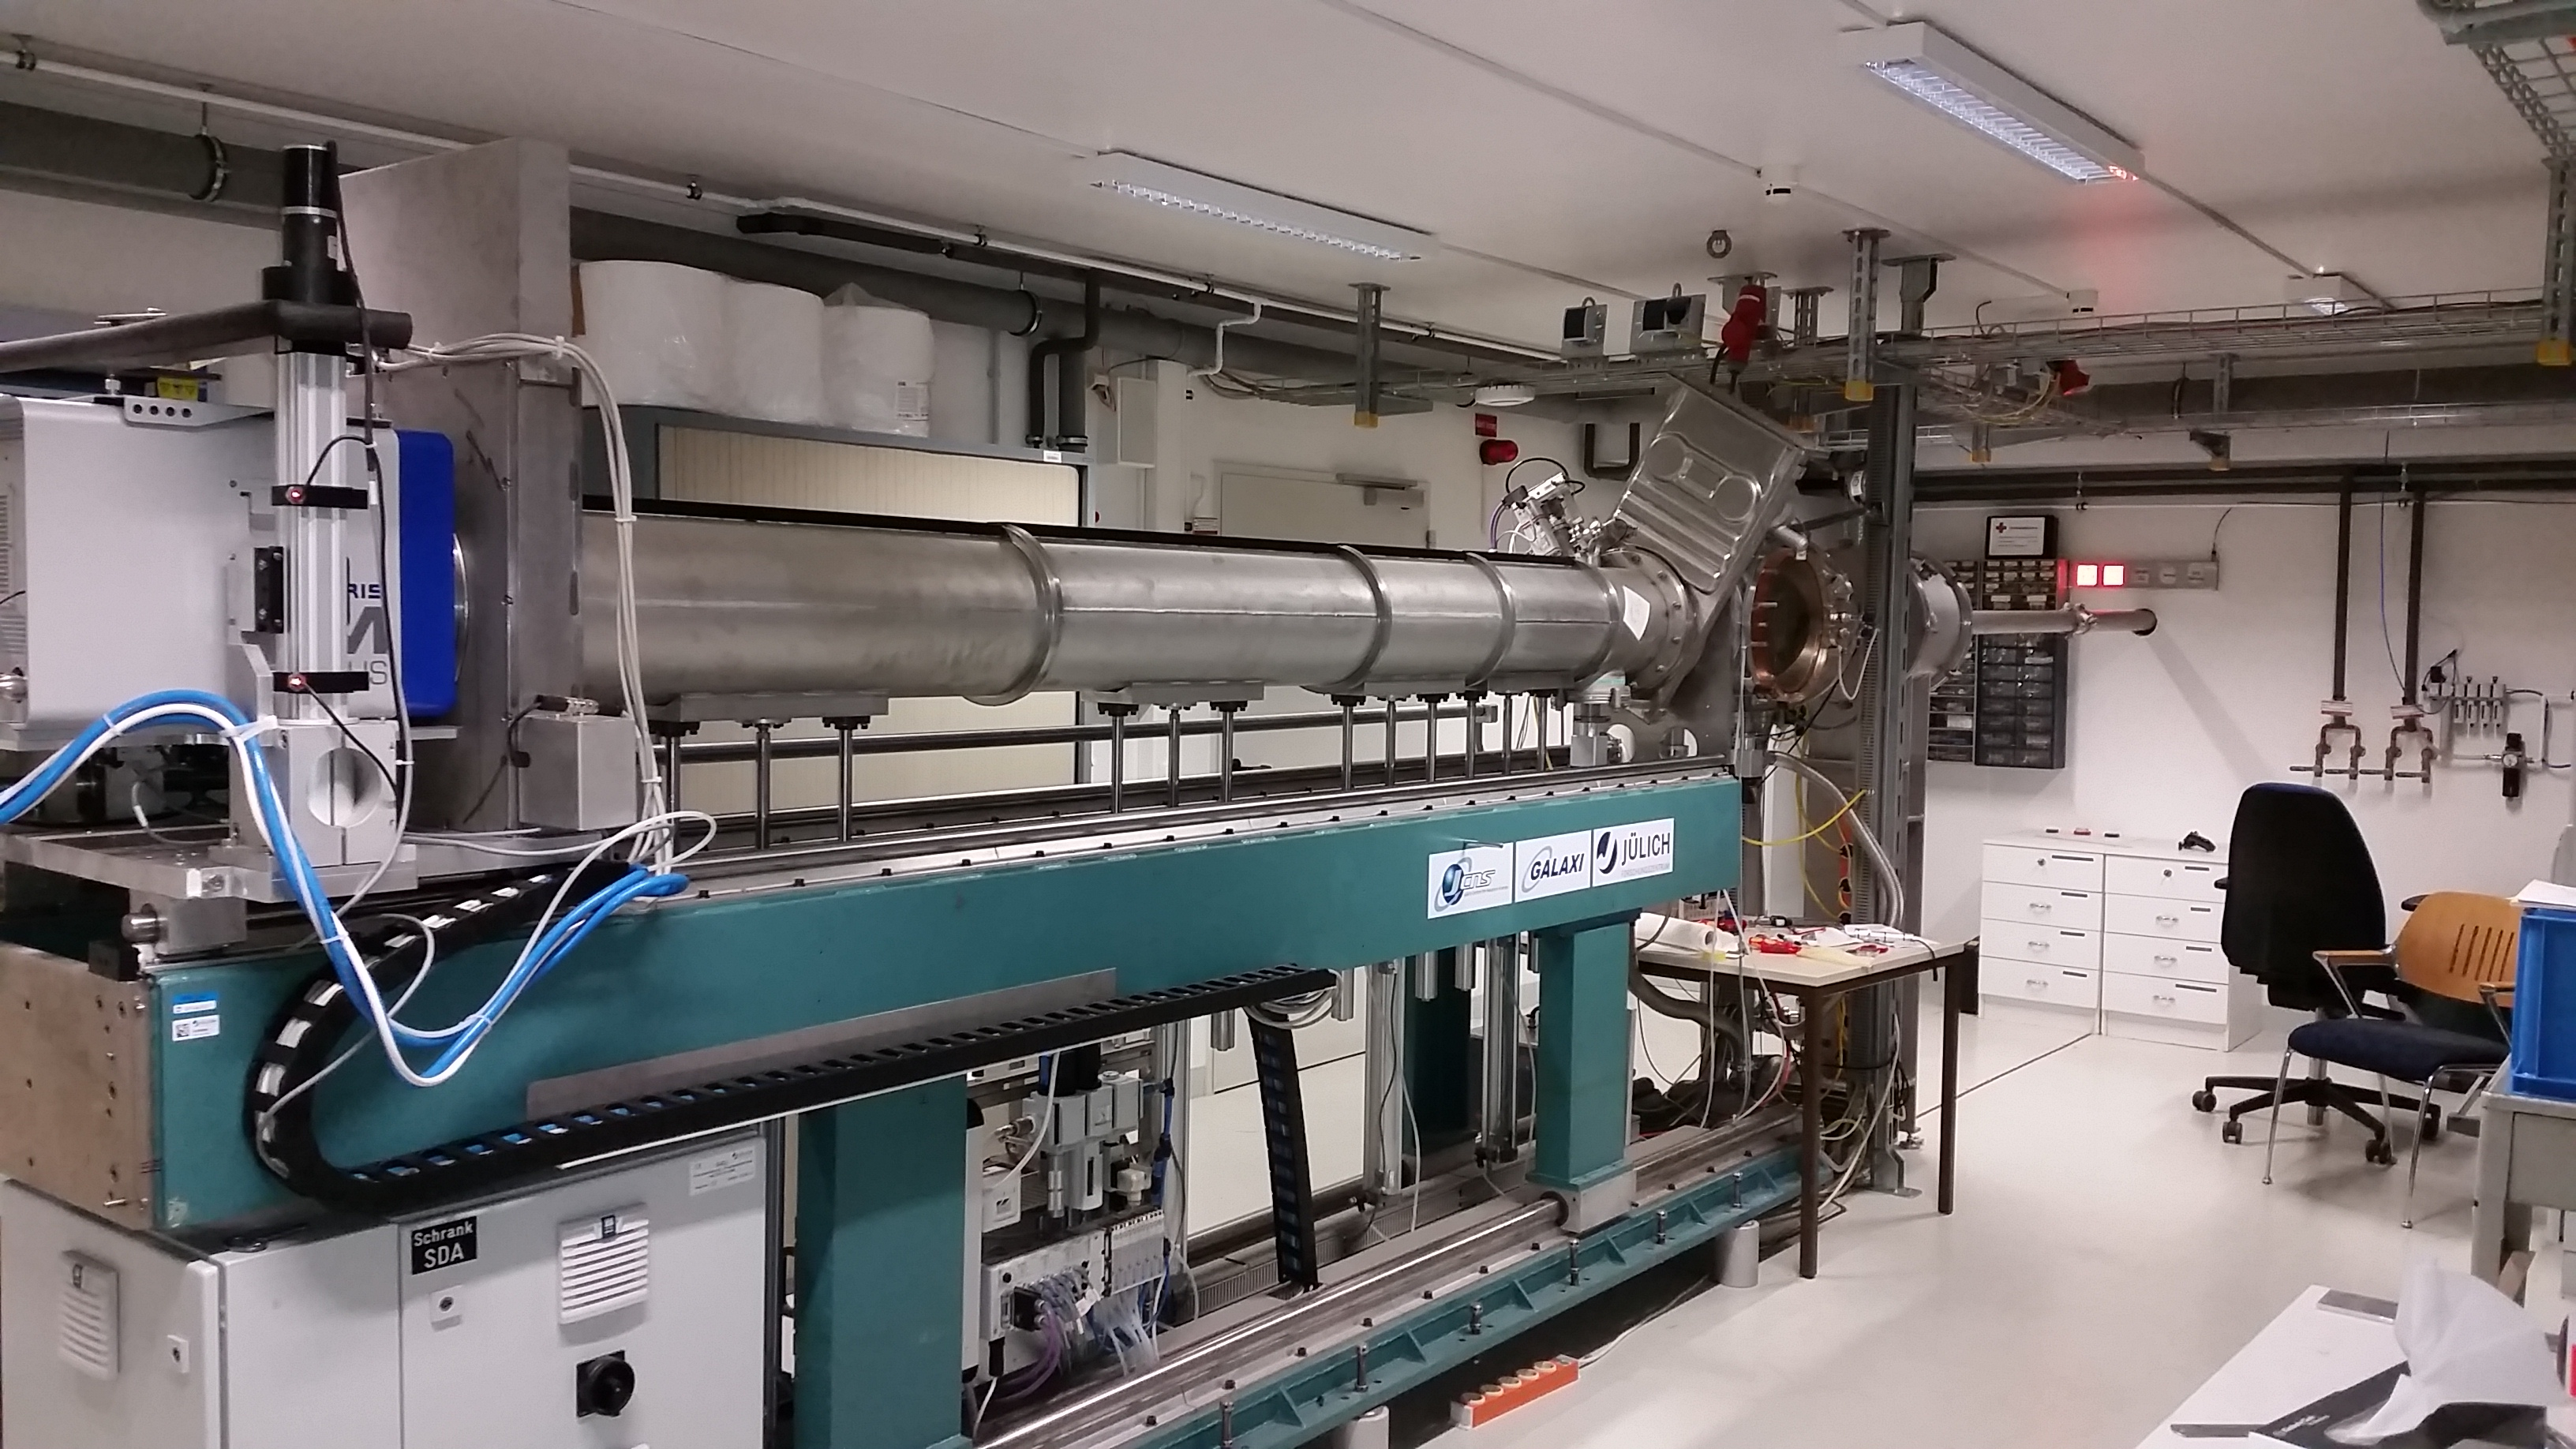
\includegraphics[width=0.7\textwidth]{instruments_galaxi}
      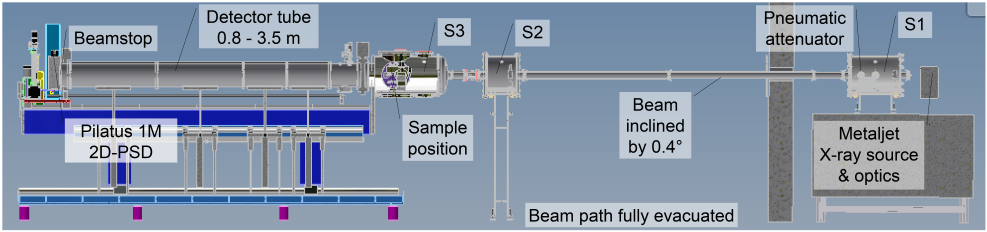
\includegraphics[width=0.7\textwidth]{appendix_instruments_GALAXISetup}
      \caption{\label{fig:lss:galaxi}GALAXI at \textsc{Forschungszentrum J\"ulich}, usable for (grazing incidence) small angle X-ray scattering and X-ray reflectometry (schematics reproduced from \cite{FZJ_2016_GALAX}).}
    \end{figure}

    The Gallium Anode Low-Angle X-ray Instrument (GALAXI) at the \textsc{Forschungszentrum J\"ulich} is set up with a liquid metal jet source and a position-sensitive Pilatus 1M detector and can be used for (grazing incidence) small-angle X-ray scattering and X-ray reflectometry \cite{FZJ_2016_GALAX}.
    By using a circulating and continuously cooled metal jet of a GaInSn metal alloy, a high flux of X-ray photons is produced, comparable to a second generation synchrotron.
    The K$\alpha$ wavelength is $\lambda \eq 1.34 \unit{\angstrom}$ and the sample-to-detector distance can be varied incrementally in five steps from $0.8 - 3.5 \unit{m}$.
    For the Pilatus 1M detector with a size of $169 \unit{mm} \times 179 \unit{mm}$ and pixel size of $172 \unit{\musf m}$.
    This results in an accessible $q$-range of $4 \cdot 10^{-2} \ldots 10 \unit{nm}^{-1}$ with the beam directed to the center of the detector and the ten innermost pixels masked by the beam stop.

    For the control of the instrument and it's motors, the Network Integrated COntrol System (NICOS) software from MLZ is used, where the experimental sequences are programmed in the Python programming language.
    The detector images are obtained as a combination of a TIF file containing the counts of the individual pixels and a text file containing motor parameters.
    Both can and have been treated by using the public Python packages as described in the respective chapters for SAXS (\refch{ch:methods:saxs}) and GISAXS(\refch{ch:methods:gisaxs}).

    \begin{figure}[ht]
      \centering
      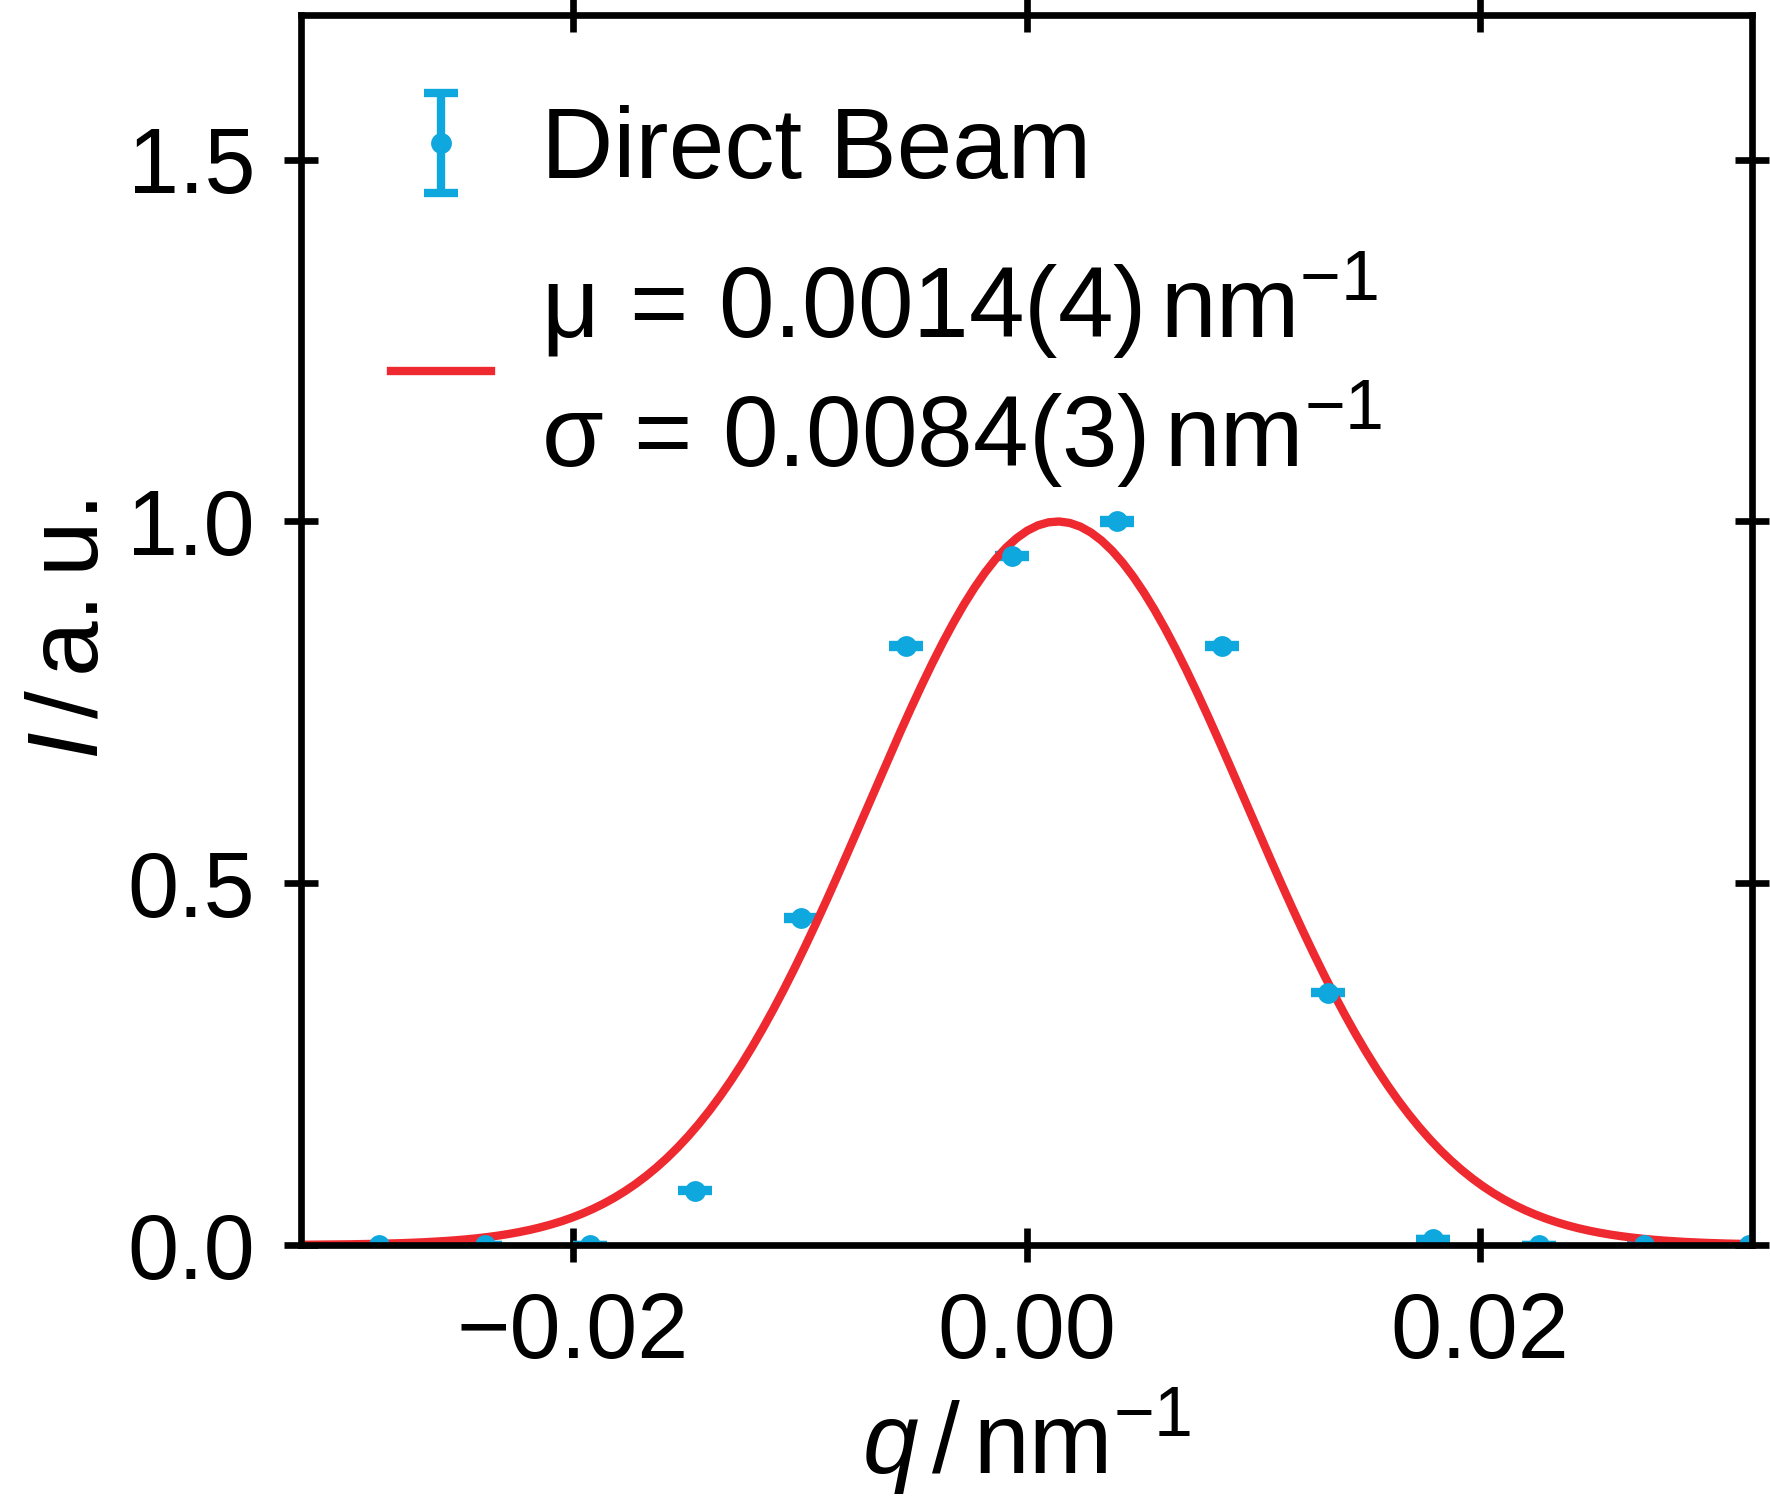
\includegraphics{appendix_instruments_GALAXIDirectBeam}
      \caption{\label{fig:lss:galaxi:directBeam}Direct beam width measured at GALAXI for slit widths of $s_2 \eq 0.5 \unit{mm}$ and $s_3 \eq 0.9 \unit{mm}$ with the detector set to a distance of $L \eq 1.73 \unit{m}$.}
    \end{figure}
    To quantify the beam divergence of the instrument, the beam width of the attenuated direct beam has been determined in \reffig{fig:lss:galaxi:directBeam}.
    The width of the direct beam is determined by a Gaussian fit to $\sigma_q \eq 0.0084(3) \unit{nm^{-1}}$, which corresponds to a FWHM of $\gamma_q \eq 0.0198(7) \unit{nm^{-1}}$.

    This value can be understood by the collimation of the system as presented in \refch{ch:methods:sans}.
    The shown direct beam is measured at a sample-to-detector distance of $L_\mathrm{SSD} \eq 1.73 \unit{m}$ for a collimation slit width of $w_c \eq 0.5 \unit{mm}$ and a sample collimation of $w_s \eq 0.5 \unit{mm}$, which are separated by $L_\mathrm{CSD} \eq 4 \unit{m}$.
    Using \refeq{eq:methods:sans:instrumentalResolution} to determine by the first two addends the contribution of the collimation to the instrumental resolution, it is evaluated to $\sigma_q^\mathrm{collimation} \approx 0.01 \unit{nm^{-1}}$, which is close to the Gaussian beam width.
    The contribution by the finite size of the pixel is on the other hand negligible in comparison with $\sigma_q^\mathrm{pixel} \approx 0.001 \unit{nm^{-1}}$.
\end{document}